\documentclass[10pt]{article}
% Final report of the 11-785 course project, organised by the course rubric.
% Numbers marked \pd{...} come from pd_numbers.tex (make_report_numbers.py) and
% fr_numbers.tex (make_final_numbers.py); tables pd_table_* and fr_table_* likewise.
\usepackage[letterpaper,textwidth=5.5in,textheight=9in,top=1in,headheight=12pt,headsep=25pt,footskip=30pt]{geometry}
\usepackage[T1]{fontenc}
\usepackage[utf8]{inputenc}
\usepackage{mathptmx}
\usepackage{amsmath,amssymb,bm}
\usepackage{microtype}
\usepackage{booktabs}
\usepackage{graphicx}
\usepackage{xcolor}
\usepackage[numbers,sort&compress]{natbib}
\usepackage[small,labelfont=bf]{caption}
\usepackage{enumitem}
\usepackage{tabularx}
\usepackage[colorlinks=true,linkcolor=blue!50!black,citecolor=blue!50!black,urlcolor=blue!50!black]{hyperref}
\setlist{nosep,leftmargin=1.4em}
\setlength{\textfloatsep}{7pt plus 2pt minus 2pt}
\setlength{\floatsep}{6pt plus 2pt minus 2pt}
\setlength{\intextsep}{6pt plus 2pt minus 2pt}
\captionsetup{skip=4pt}
\renewcommand{\topfraction}{0.95}
\renewcommand{\bottomfraction}{0.6}
\renewcommand{\textfraction}{0.06}
\renewcommand{\floatpagefraction}{0.85}
\setcounter{topnumber}{3}
\setcounter{totalnumber}{4}
\newcommand{\repo}{\url{https://github.com/chilalaabubakar/IDL-PROJECT}}
\makeatletter
\newcommand{\pd}[1]{\@ifundefined{pd@#1}{\textcolor{red}{[#1]}}{\csname pd@#1\endcsname}}
\newcommand{\pdset}[2]{\expandafter\gdef\csname pd@#1\endcsname{#2}}
\@secpenalty=0 % do not end a page early just because a section follows
\makeatother
\IfFileExists{pd_numbers.tex}{% written by make_report_numbers.py
\pdset{abl-diff-layers1}{6.2}
\pdset{abl-diff-layers2}{1.3}
\pdset{abl-diff-no-weights}{1.2}
\pdset{abl-diff-real-only}{0.0}
\pdset{abl-diff-scratch}{22.0}
\pdset{abl-label-layers1-interstitial}{0}
\pdset{abl-label-layers1-vacancy}{0}
\pdset{abl-label-layers2-interstitial}{0}
\pdset{abl-label-layers2-vacancy}{0}
\pdset{abl-label-no-weights-interstitial}{0}
\pdset{abl-label-no-weights-vacancy}{7}
\pdset{abl-label-real-only-interstitial}{17}
\pdset{abl-label-real-only-vacancy}{32}
\pdset{abl-label-reference-interstitial}{18}
\pdset{abl-label-reference-vacancy}{27}
\pdset{abl-label-scratch-interstitial}{0}
\pdset{abl-label-scratch-vacancy}{0}
\pdset{abl-layers1-all}{15.6}
\pdset{abl-layers1-antisite}{14.2}
\pdset{abl-layers1-frenkel}{13.8}
\pdset{abl-layers1-high}{17.3}
\pdset{abl-layers1-interstitial}{21.8}
\pdset{abl-layers1-low}{14.8}
\pdset{abl-layers1-sd}{1.5}
\pdset{abl-layers1-vacancy}{12.3}
\pdset{abl-layers2-all}{20.6}
\pdset{abl-layers2-antisite}{20.8}
\pdset{abl-layers2-frenkel}{21.3}
\pdset{abl-layers2-high}{23.1}
\pdset{abl-layers2-interstitial}{26.5}
\pdset{abl-layers2-low}{18.3}
\pdset{abl-layers2-sd}{2.4}
\pdset{abl-layers2-vacancy}{13.8}
\pdset{abl-lower-layers1}{3}
\pdset{abl-lower-layers2}{3}
\pdset{abl-lower-no-weights}{3}
\pdset{abl-lower-real-only}{2}
\pdset{abl-lower-scratch}{3}
\pdset{abl-no-weights-all}{42.7}
\pdset{abl-no-weights-antisite}{39.5}
\pdset{abl-no-weights-frenkel}{35.1}
\pdset{abl-no-weights-high}{43.5}
\pdset{abl-no-weights-interstitial}{31.0}
\pdset{abl-no-weights-low}{41.6}
\pdset{abl-no-weights-sd}{1.0}
\pdset{abl-no-weights-vacancy}{63.2}
\pdset{abl-real-only-ahead}{2.5}
\pdset{abl-real-only-all}{43.8}
\pdset{abl-real-only-antisite}{40.2}
\pdset{abl-real-only-behind}{2.5}
\pdset{abl-real-only-frenkel}{38.0}
\pdset{abl-real-only-high}{46.1}
\pdset{abl-real-only-interstitial}{30.8}
\pdset{abl-real-only-low}{42.1}
\pdset{abl-real-only-sd}{2.1}
\pdset{abl-real-only-vacancy}{64.7}
\pdset{abl-reference-all}{43.8}
\pdset{abl-reference-antisite}{41.7}
\pdset{abl-reference-frenkel}{38.7}
\pdset{abl-reference-high}{44.7}
\pdset{abl-reference-interstitial}{30.7}
\pdset{abl-reference-low}{43.2}
\pdset{abl-reference-sd}{0.8}
\pdset{abl-reference-vacancy}{63.0}
\pdset{abl-scratch-all}{21.9}
\pdset{abl-scratch-antisite}{24.2}
\pdset{abl-scratch-frenkel}{22.2}
\pdset{abl-scratch-high}{23.7}
\pdset{abl-scratch-interstitial}{26.8}
\pdset{abl-scratch-low}{18.7}
\pdset{abl-scratch-sd}{2.8}
\pdset{abl-scratch-vacancy}{14.3}
\pdset{abl-seeds}{three}
\pdset{abl-updates}{2,000}
\pdset{chance-antisite}{4}
\pdset{chance-frenkel}{5.4}
\pdset{chance-interstitial}{3}
\pdset{chance-max}{5}
\pdset{chance-min}{3}
\pdset{chance-vacancy}{2.9}
\pdset{exp-20k}{50.3}
\pdset{exp-60k}{54}
\pdset{exp-p-cal}{$p<0.001$}
\pdset{exp-p-length}{$p=0.001$}
\pdset{exp-uncal}{50.7}
\pdset{fin-by-all}{36--37}
\pdset{fin-by-none}{36--38}
\pdset{fin-by-one}{62--64}
\pdset{fin-cnn-all}{54.0}
\pdset{fin-cnn-antisite}{52.8}
\pdset{fin-cnn-frenkel}{38.4}
\pdset{fin-cnn-high}{54.4}
\pdset{fin-cnn-hours}{0.6}
\pdset{fin-cnn-interstitial}{51.2}
\pdset{fin-cnn-low}{53.5}
\pdset{fin-cnn-noshift}{12}
\pdset{fin-cnn-shift}{88}
\pdset{fin-cnn-size}{0.50}
\pdset{fin-cnn-vacancy}{69.7}
\pdset{fin-cnn3-all}{54.7}
\pdset{fin-cnn3-antisite}{54.0}
\pdset{fin-cnn3-frenkel}{38.7}
\pdset{fin-cnn3-hi}{59}
\pdset{fin-cnn3-interstitial}{51.5}
\pdset{fin-cnn3-lo}{51}
\pdset{fin-cnn3-p}{$p=0.86$}
\pdset{fin-cnn3-vacancy}{70.5}
\pdset{fin-egnn-all}{43.5}
\pdset{fin-egnn-antisite}{44.0}
\pdset{fin-egnn-frenkel}{35.1}
\pdset{fin-egnn-high}{43.9}
\pdset{fin-egnn-hours}{0.8}
\pdset{fin-egnn-interstitial}{29.7}
\pdset{fin-egnn-low}{42.9}
\pdset{fin-egnn-noshift}{0}
\pdset{fin-egnn-shift}{100}
\pdset{fin-egnn-size}{0.52}
\pdset{fin-egnn-vacancy}{63.2}
\pdset{fin-egnn3-all}{44.0}
\pdset{fin-egnn3-antisite}{45.5}
\pdset{fin-egnn3-frenkel}{32.7}
\pdset{fin-egnn3-hi}{48}
\pdset{fin-egnn3-interstitial}{30.0}
\pdset{fin-egnn3-lo}{40}
\pdset{fin-egnn3-p}{$p=1.00$}
\pdset{fin-egnn3-vacancy}{65.0}
\pdset{fin-lost-cnn}{38--42}
\pdset{fin-lost-pre}{43}
\pdset{fin-lost-tr}{34--41}
\pdset{fin-main-all}{54.0}
\pdset{fin-main-antisite}{49.0}
\pdset{fin-main-frenkel}{45.3}
\pdset{fin-main-interstitial}{50.0}
\pdset{fin-main-noshift}{0}
\pdset{fin-main-shift}{100}
\pdset{fin-main-size}{0.52}
\pdset{fin-main-vacancy}{69.5}
\pdset{fin-only-cnn}{114--122}
\pdset{fin-only-pre}{91}
\pdset{fin-only-tr}{110--116}
\pdset{fin-p-cnn}{$p<0.001$}
\pdset{fin-p-pre}{$p<0.001$}
\pdset{fin-p-tr}{$p<0.001$}
\pdset{fin-p-tr-cnn}{$p=0.49$--$0.91$}
\pdset{fin-p-tr-cnn-antisite}{0.33}
\pdset{fin-p-tr-cnn-frenkel}{0.25}
\pdset{fin-p-tr-cnn-interstitial}{0.04}
\pdset{fin-p-tr-cnn-vacancy}{0.12}
\pdset{fin-pair-all}{55.2}
\pdset{fin-pair-antisite}{55.5}
\pdset{fin-pair-frenkel}{41.3}
\pdset{fin-pair-hi}{59}
\pdset{fin-pair-interstitial}{51.5}
\pdset{fin-pair-lo}{51}
\pdset{fin-pair-p}{$p=0.090$}
\pdset{fin-pair-vacancy}{69.0}
\pdset{fin-pre-all}{50.3}
\pdset{fin-pre-antisite}{46.5}
\pdset{fin-pre-frenkel}{36.7}
\pdset{fin-pre-interstitial}{47.5}
\pdset{fin-pre-noshift}{0}
\pdset{fin-pre-shift}{100}
\pdset{fin-pre-size}{0.52}
\pdset{fin-pre-vacancy}{67.0}
\pdset{fin-report-all}{55.2}
\pdset{fin-report-antisite}{55.0}
\pdset{fin-report-frenkel}{41.3}
\pdset{fin-report-hi}{59}
\pdset{fin-report-interstitial}{51.0}
\pdset{fin-report-lo}{51}
\pdset{fin-report-p}{$p=0.30$}
\pdset{fin-report-vacancy}{70.0}
\pdset{fin-six-all}{55.1}
\pdset{fin-six-antisite}{56.0}
\pdset{fin-six-frenkel}{41.3}
\pdset{fin-six-hi}{59}
\pdset{fin-six-interstitial}{49.5}
\pdset{fin-six-lo}{51}
\pdset{fin-six-p}{$p=0.58$}
\pdset{fin-six-vacancy}{70.0}
\pdset{fin-three-all}{54.1}
\pdset{fin-three-antisite}{54.5}
\pdset{fin-three-frenkel}{40.7}
\pdset{fin-three-hi}{58}
\pdset{fin-three-interstitial}{50.0}
\pdset{fin-three-lo}{50}
\pdset{fin-three-p}{$p=0.77$}
\pdset{fin-three-vacancy}{68.0}
\pdset{fin-tr-all}{53.6}
\pdset{fin-tr-antisite}{54.2}
\pdset{fin-tr-frenkel}{42.0}
\pdset{fin-tr-high}{53.9}
\pdset{fin-tr-hours}{0.6}
\pdset{fin-tr-interstitial}{48.3}
\pdset{fin-tr-low}{53.3}
\pdset{fin-tr-noshift}{0}
\pdset{fin-tr-shift}{100}
\pdset{fin-tr-size}{0.58}
\pdset{fin-tr-vacancy}{67.2}
\pdset{fin-tr3-all}{54.5}
\pdset{fin-tr3-antisite}{56.5}
\pdset{fin-tr3-frenkel}{42.7}
\pdset{fin-tr3-hi}{58}
\pdset{fin-tr3-interstitial}{48.0}
\pdset{fin-tr3-lo}{51}
\pdset{fin-tr3-p}{$p=0.44$}
\pdset{fin-tr3-vacancy}{68.0}
\pdset{fother-found-bonds}{26.2}
\pdset{fother-found-bonds-hi}{36}
\pdset{fother-found-bonds-lo}{17}
\pdset{fother-found-energy}{31}
\pdset{fother-found-energy-hi}{41}
\pdset{fother-found-energy-lo}{22}
\pdset{fother-found-finder}{44}
\pdset{fother-found-finder-hi}{55}
\pdset{fother-found-finder-lo}{33}
\pdset{fother-found-geometry}{20.2}
\pdset{fother-found-geometry-hi}{28}
\pdset{fother-found-geometry-lo}{12}
\pdset{fother-n}{84}
\pdset{fother-p-found-energy}{$p=0.071$}
\pdset{fother-p-restored-energy}{$p=0.77$}
\pdset{fother-restored-bonds}{1.2}
\pdset{fother-restored-bonds-hi}{4}
\pdset{fother-restored-bonds-lo}{0}
\pdset{fother-restored-ceiling}{27.4}
\pdset{fother-restored-ceiling-hi}{38}
\pdset{fother-restored-ceiling-lo}{18}
\pdset{fother-restored-energy}{6}
\pdset{fother-restored-energy-hi}{11}
\pdset{fother-restored-energy-lo}{1}
\pdset{fother-restored-finder}{8.3}
\pdset{fother-restored-finder-hi}{14}
\pdset{fother-restored-finder-lo}{3}
\pdset{fother-restored-geometry}{0}
\pdset{fother-restored-geometry-hi}{4}
\pdset{fother-restored-geometry-lo}{0}
\pdset{found-best-antisite}{31.5}
\pdset{found-best-frenkel}{32.7}
\pdset{found-best-interstitial}{28}
\pdset{found-best-vacancy}{47.5}
\pdset{found-bonds-antisite}{31.5}
\pdset{found-bonds-frenkel}{27.3}
\pdset{found-bonds-interstitial}{28}
\pdset{found-bonds-max}{31.5}
\pdset{found-bonds-min}{27.3}
\pdset{found-bonds-vacancy}{29}
\pdset{found-energy-antisite}{29}
\pdset{found-energy-frenkel}{32.7}
\pdset{found-energy-interstitial}{28}
\pdset{found-energy-max}{32.7}
\pdset{found-energy-min}{28}
\pdset{found-energy-vacancy}{29.5}
\pdset{found-finder-antisite}{49}
\pdset{found-finder-frenkel}{45.3}
\pdset{found-finder-interstitial}{50}
\pdset{found-finder-vacancy}{69.5}
\pdset{found-geometry-antisite}{16.5}
\pdset{found-geometry-frenkel}{26.7}
\pdset{found-geometry-interstitial}{15}
\pdset{found-geometry-max}{47.5}
\pdset{found-geometry-min}{15}
\pdset{found-geometry-vacancy}{47.5}
\pdset{fp-n-anti}{35}
\pdset{fp-n-close}{27}
\pdset{fp-n-complex}{19}
\pdset{fp-n-none}{3}
\pdset{fp-n-pair}{66}
\pdset{fp-n-pair-pure}{40}
\pdset{fpair-found-bonds}{28.8}
\pdset{fpair-found-bonds-hi}{40}
\pdset{fpair-found-bonds-lo}{19}
\pdset{fpair-found-energy}{34.8}
\pdset{fpair-found-energy-hi}{47}
\pdset{fpair-found-energy-lo}{24}
\pdset{fpair-found-finder}{47}
\pdset{fpair-found-finder-hi}{59}
\pdset{fpair-found-finder-lo}{35}
\pdset{fpair-found-geometry}{34.8}
\pdset{fpair-found-geometry-hi}{47}
\pdset{fpair-found-geometry-lo}{24}
\pdset{fpair-n}{66}
\pdset{fpair-p-found-energy}{$p=0.15$}
\pdset{fpair-p-restored-energy}{$p=0.18$}
\pdset{fpair-restored-bonds}{1.5}
\pdset{fpair-restored-bonds-hi}{5}
\pdset{fpair-restored-bonds-lo}{0}
\pdset{fpair-restored-ceiling}{60.6}
\pdset{fpair-restored-ceiling-hi}{71}
\pdset{fpair-restored-ceiling-lo}{49}
\pdset{fpair-restored-energy}{9.1}
\pdset{fpair-restored-energy-hi}{17}
\pdset{fpair-restored-energy-lo}{3}
\pdset{fpair-restored-finder}{18.2}
\pdset{fpair-restored-finder-hi}{28}
\pdset{fpair-restored-finder-lo}{10}
\pdset{fpair-restored-geometry}{0}
\pdset{fpair-restored-geometry-hi}{5}
\pdset{fpair-restored-geometry-lo}{0}
\pdset{frenkel-exact-energy}{7}
\pdset{frenkel-exact-finder}{21}
\pdset{gap-finder-energy-max}{40}
\pdset{gap-finder-energy-min}{20}
\pdset{glass-auc}{0.75}
\pdset{glass-clean-cal}{2}
\pdset{glass-clean-raw}{68}
\pdset{glass-def-cal}{28.7}
\pdset{lead-found-antisite}{18}
\pdset{lead-found-frenkel}{13}
\pdset{lead-found-interstitial}{22}
\pdset{lead-found-max}{22}
\pdset{lead-found-min}{18}
\pdset{lead-found-vacancy}{22}
\pdset{lead-restored-antisite}{22}
\pdset{lead-restored-frenkel}{5}
\pdset{lead-restored-interstitial}{16}
\pdset{lead-restored-vacancy}{13}
\pdset{n-antisite}{200}
\pdset{n-frenkel}{150}
\pdset{n-interstitial}{200}
\pdset{n-test}{750}
\pdset{n-tests-family}{12}
\pdset{n-vacancy}{200}
\pdset{occ-anti}{71}
\pdset{occ-anti-pairlike}{22}
\pdset{occ-int}{95.5}
\pdset{occ-undone}{50}
\pdset{occ-undone-n}{50}
\pdset{occ-vac}{93}
\pdset{p-found-bonds-antisite}{<0.001}
\pdset{p-found-bonds-frenkel}{<0.001}
\pdset{p-found-bonds-interstitial}{<0.001}
\pdset{p-found-bonds-vacancy}{<0.001}
\pdset{p-found-energy-antisite}{<0.001}
\pdset{p-found-energy-frenkel}{0.014}
\pdset{p-found-energy-interstitial}{<0.001}
\pdset{p-found-energy-vacancy}{<0.001}
\pdset{p-found-geometry-antisite}{<0.001}
\pdset{p-found-geometry-frenkel}{0.002}
\pdset{p-found-geometry-interstitial}{<0.001}
\pdset{p-found-geometry-vacancy}{<0.001}
\pdset{p-restored-bonds-antisite}{<0.001}
\pdset{p-restored-bonds-frenkel}{<0.001}
\pdset{p-restored-bonds-interstitial}{<0.001}
\pdset{p-restored-bonds-vacancy}{<0.001}
\pdset{p-restored-energy-antisite}{<0.001}
\pdset{p-restored-energy-frenkel}{0.169}
\pdset{p-restored-energy-interstitial}{<0.001}
\pdset{p-restored-energy-vacancy}{<0.001}
\pdset{p-restored-geometry-antisite}{<0.001}
\pdset{p-restored-geometry-frenkel}{<0.001}
\pdset{p-restored-geometry-interstitial}{<0.001}
\pdset{p-restored-geometry-vacancy}{<0.001}
\pdset{p-worst-found}{p<0.001}
\pdset{p-worst-restored}{p<0.001}
\pdset{praw-found-bonds-antisite}{<0.001}
\pdset{praw-found-bonds-frenkel}{<0.001}
\pdset{praw-found-bonds-interstitial}{<0.001}
\pdset{praw-found-bonds-vacancy}{<0.001}
\pdset{praw-found-energy-antisite}{<0.001}
\pdset{praw-found-energy-frenkel}{0.014}
\pdset{praw-found-energy-interstitial}{<0.001}
\pdset{praw-found-energy-vacancy}{<0.001}
\pdset{praw-found-geometry-antisite}{<0.001}
\pdset{praw-found-geometry-frenkel}{<0.001}
\pdset{praw-found-geometry-interstitial}{<0.001}
\pdset{praw-found-geometry-vacancy}{<0.001}
\pdset{praw-restored-bonds-antisite}{<0.001}
\pdset{praw-restored-bonds-frenkel}{<0.001}
\pdset{praw-restored-bonds-interstitial}{<0.001}
\pdset{praw-restored-bonds-vacancy}{<0.001}
\pdset{praw-restored-energy-antisite}{<0.001}
\pdset{praw-restored-energy-frenkel}{0.169}
\pdset{praw-restored-energy-interstitial}{<0.001}
\pdset{praw-restored-energy-vacancy}{<0.001}
\pdset{praw-restored-geometry-antisite}{<0.001}
\pdset{praw-restored-geometry-frenkel}{<0.001}
\pdset{praw-restored-geometry-interstitial}{<0.001}
\pdset{praw-restored-geometry-vacancy}{<0.001}
\pdset{press-antisite}{16}
\pdset{press-antisite-hi}{22}
\pdset{press-antisite-lo}{11}
\pdset{press-antisite-rule}{lowest}
\pdset{press-frenkel}{10.7}
\pdset{press-frenkel-hi}{16}
\pdset{press-frenkel-lo}{6}
\pdset{press-frenkel-rule}{lowest}
\pdset{press-interstitial}{19}
\pdset{press-interstitial-hi}{25}
\pdset{press-interstitial-lo}{14}
\pdset{press-interstitial-rule}{most unusual}
\pdset{press-max}{19}
\pdset{press-min}{8.5}
\pdset{press-p-antisite}{$p<0.001$}
\pdset{press-p-frenkel}{$p<0.001$}
\pdset{press-p-interstitial}{$p<0.001$}
\pdset{press-p-vacancy}{$p<0.001$}
\pdset{press-ref-a}{6.5\pm5.4}
\pdset{press-ref-b}{2.9\pm5.4}
\pdset{press-vacancy}{8.5}
\pdset{press-vacancy-hi}{12}
\pdset{press-vacancy-lo}{5}
\pdset{press-vacancy-rule}{lowest}
\pdset{press-val-highest}{21}
\pdset{press-val-unusual}{21.5}
\pdset{presscell-antisite}{15}
\pdset{presscell-antisite-hi}{20}
\pdset{presscell-antisite-lo}{10}
\pdset{presscell-antisite-rule}{lowest}
\pdset{presscell-frenkel}{7.3}
\pdset{presscell-frenkel-hi}{12}
\pdset{presscell-frenkel-lo}{3}
\pdset{presscell-frenkel-rule}{lowest}
\pdset{presscell-interstitial}{16.5}
\pdset{presscell-interstitial-hi}{23}
\pdset{presscell-interstitial-lo}{10}
\pdset{presscell-interstitial-rule}{highest}
\pdset{presscell-max}{16.5}
\pdset{presscell-min}{7}
\pdset{presscell-p-antisite}{$p<0.001$}
\pdset{presscell-p-frenkel}{$p<0.001$}
\pdset{presscell-p-interstitial}{$p<0.001$}
\pdset{presscell-p-vacancy}{$p<0.001$}
\pdset{presscell-vacancy}{7}
\pdset{presscell-vacancy-hi}{10}
\pdset{presscell-vacancy-lo}{4}
\pdset{presscell-vacancy-rule}{lowest}
\pdset{ratio-finder-energy-max}{2.4}
\pdset{ratio-finder-energy-min}{1.7}
\pdset{repair-overlap-1}{1--40}
\pdset{repair-overlap-10}{50--73}
\pdset{repair-removed-v1}{7--9}
\pdset{repair-removed-v2}{13--16}
\pdset{restored-best-antisite}{8}
\pdset{restored-best-frenkel}{7.3}
\pdset{restored-best-interstitial}{21.5}
\pdset{restored-best-vacancy}{40.5}
\pdset{restored-bonds-antisite}{7.5}
\pdset{restored-bonds-frenkel}{1.3}
\pdset{restored-bonds-interstitial}{21.5}
\pdset{restored-bonds-max}{22}
\pdset{restored-bonds-min}{1.3}
\pdset{restored-bonds-vacancy}{22}
\pdset{restored-ceiling-antisite}{68.5}
\pdset{restored-ceiling-frenkel}{42}
\pdset{restored-ceiling-interstitial}{80}
\pdset{restored-ceiling-max}{80}
\pdset{restored-ceiling-min}{42}
\pdset{restored-ceiling-vacancy}{67}
\pdset{restored-energy-antisite}{8}
\pdset{restored-energy-frenkel}{7.3}
\pdset{restored-energy-interstitial}{21}
\pdset{restored-energy-max}{26}
\pdset{restored-energy-min}{7.3}
\pdset{restored-energy-vacancy}{26}
\pdset{restored-finder-antisite}{30}
\pdset{restored-finder-frenkel}{12.7}
\pdset{restored-finder-interstitial}{38}
\pdset{restored-finder-vacancy}{53.5}
\pdset{restored-geometry-antisite}{1.5}
\pdset{restored-geometry-frenkel}{0}
\pdset{restored-geometry-interstitial}{8.5}
\pdset{restored-geometry-max}{40.5}
\pdset{restored-geometry-min}{0}
\pdset{restored-geometry-vacancy}{40.5}
\pdset{seed-agree}{88}
\pdset{seed-by-all}{37.7}
\pdset{seed-by-none}{50.1}
\pdset{seed-ensemble}{45.1}
\pdset{seed-ref-runs}{43.2, 43.6 and 44.7}
\pdset{stab-cnn-clipped}{85}
\pdset{stab-cnn-gspikes}{0}
\pdset{stab-cnn-largest}{6.3--8.1}
\pdset{stab-cnn-lspikes}{0}
\pdset{stab-cnn-median}{1.6--1.8}
\pdset{stab-cnn-runs}{3}
\pdset{stab-cnn-updates}{20,000}
\pdset{stab-egnn-clipped}{85--88}
\pdset{stab-egnn-cut}{85--96}
\pdset{stab-egnn-first}{7,818 and 9,704}
\pdset{stab-egnn-gspikes}{71--131}
\pdset{stab-egnn-largest}{55--82}
\pdset{stab-egnn-lspikes}{14--34}
\pdset{stab-egnn-median}{1.5--1.6}
\pdset{stab-egnn-runs}{3}
\pdset{stab-egnn-updates}{20,000}
\pdset{stab-max-ratio}{46}
\pdset{stab-not-finite}{0}
\pdset{stab-now-clipped}{1--3}
\pdset{stab-now-first}{647 and 731}
\pdset{stab-now-gspikes}{3--4}
\pdset{stab-now-largest}{6.2--6.7}
\pdset{stab-now-lspikes}{5--11}
\pdset{stab-now-median}{0.31--0.34}
\pdset{stab-now-runs}{2}
\pdset{stab-now-updates}{2,000}
\pdset{stab-ref-clipped}{95--96}
\pdset{stab-ref-first}{395 and 811}
\pdset{stab-ref-gspikes}{9--32}
\pdset{stab-ref-largest}{38--86}
\pdset{stab-ref-lspikes}{1--13}
\pdset{stab-ref-median}{2.0--2.5}
\pdset{stab-ref-runs}{3}
\pdset{stab-ref-updates}{2,000}
\pdset{stab-runs}{23}
\pdset{stab-scr-clipped}{92--93}
\pdset{stab-scr-gspikes}{0}
\pdset{stab-scr-largest}{4.1--5.2}
\pdset{stab-scr-lspikes}{0}
\pdset{stab-scr-median}{1.4--1.5}
\pdset{stab-scr-runs}{3}
\pdset{stab-scr-updates}{2,000}
\pdset{stab-tr-clipped}{40--50}
\pdset{stab-tr-gspikes}{0}
\pdset{stab-tr-largest}{4.9--5.5}
\pdset{stab-tr-lspikes}{0--1}
\pdset{stab-tr-median}{0.9--1.0}
\pdset{stab-tr-runs}{3}
\pdset{stab-tr-updates}{20,000}
\pdset{vacA-found-bonds}{40.9}
\pdset{vacA-found-bonds-hi}{49}
\pdset{vacA-found-bonds-lo}{33}
\pdset{vacA-found-energy}{40.2}
\pdset{vacA-found-energy-hi}{49}
\pdset{vacA-found-energy-lo}{31}
\pdset{vacA-found-finder}{69.3}
\pdset{vacA-found-finder-hi}{77}
\pdset{vacA-found-finder-lo}{61}
\pdset{vacA-found-geometry}{56.7}
\pdset{vacA-found-geometry-hi}{66}
\pdset{vacA-found-geometry-lo}{47}
\pdset{vacA-n}{127}
\pdset{vacA-p-found-energy}{$p<0.001$}
\pdset{vacA-p-restored-energy}{$p<0.001$}
\pdset{vacA-restored-bonds}{29.1}
\pdset{vacA-restored-bonds-hi}{38}
\pdset{vacA-restored-bonds-lo}{21}
\pdset{vacA-restored-ceiling}{58.3}
\pdset{vacA-restored-ceiling-hi}{67}
\pdset{vacA-restored-ceiling-lo}{49}
\pdset{vacA-restored-energy}{34.6}
\pdset{vacA-restored-energy-hi}{43}
\pdset{vacA-restored-energy-lo}{26}
\pdset{vacA-restored-finder}{49.6}
\pdset{vacA-restored-finder-hi}{59}
\pdset{vacA-restored-finder-lo}{40}
\pdset{vacA-restored-geometry}{47.2}
\pdset{vacA-restored-geometry-hi}{57}
\pdset{vacA-restored-geometry-lo}{38}
\pdset{vacB-found-bonds}{8.2}
\pdset{vacB-found-bonds-hi}{15}
\pdset{vacB-found-bonds-lo}{3}
\pdset{vacB-found-energy}{11}
\pdset{vacB-found-energy-hi}{18}
\pdset{vacB-found-energy-lo}{4}
\pdset{vacB-found-finder}{69.9}
\pdset{vacB-found-finder-hi}{80}
\pdset{vacB-found-finder-lo}{59}
\pdset{vacB-found-geometry}{31.5}
\pdset{vacB-found-geometry-hi}{43}
\pdset{vacB-found-geometry-lo}{20}
\pdset{vacB-n}{73}
\pdset{vacB-p-found-energy}{$p<0.001$}
\pdset{vacB-p-restored-energy}{$p<0.001$}
\pdset{vacB-restored-bonds}{9.6}
\pdset{vacB-restored-bonds-hi}{17}
\pdset{vacB-restored-bonds-lo}{4}
\pdset{vacB-restored-ceiling}{82.2}
\pdset{vacB-restored-ceiling-hi}{90}
\pdset{vacB-restored-ceiling-lo}{73}
\pdset{vacB-restored-energy}{11}
\pdset{vacB-restored-energy-hi}{18}
\pdset{vacB-restored-energy-lo}{4}
\pdset{vacB-restored-finder}{60.3}
\pdset{vacB-restored-finder-hi}{71}
\pdset{vacB-restored-finder-lo}{49}
\pdset{vacB-restored-geometry}{28.8}
\pdset{vacB-restored-geometry-hi}{40}
\pdset{vacB-restored-geometry-lo}{18}
\pdset{vacancy-closed}{40}
\pdset{vacancy-open}{60}
}{}
\IfFileExists{fr_numbers.tex}{% written by make_final_numbers.py
\pdset{feat-atoms}{4,159}
\pdset{knn-den}{31}
\pdset{knn-fin}{43}
\pdset{noise-bonds-0}{28.9}
\pdset{noise-bonds-100}{8}
\pdset{noise-bonds-20}{29.2}
\pdset{noise-bonds-50}{26.3}
\pdset{noise-cell-0}{26.4}
\pdset{noise-cell-100}{8.9}
\pdset{noise-cell-20}{22.8}
\pdset{noise-cell-50}{15.7}
\pdset{noise-cnn-0}{53.5}
\pdset{noise-cnn-100}{10.1}
\pdset{noise-cnn-20}{35.1}
\pdset{noise-cnn-50}{17.6}
\pdset{noise-drop-fin}{16}
\pdset{noise-energy-0}{29.6}
\pdset{noise-energy-100}{3.6}
\pdset{noise-energy-20}{10.4}
\pdset{noise-energy-50}{3.5}
\pdset{noise-fin-0}{54}
\pdset{noise-fin-100}{11.3}
\pdset{noise-fin-20}{38.1}
\pdset{noise-fin-50}{18.8}
\pdset{noise-max-last}{12.7}
\pdset{noise-scr-0}{43.9}
\pdset{noise-scr-100}{12.7}
\pdset{noise-scr-20}{42.4}
\pdset{noise-scr-50}{34.8}
\pdset{noise-tr-0}{53.7}
\pdset{noise-tr-100}{3.5}
\pdset{noise-tr-20}{31.1}
\pdset{noise-tr-50}{7.1}
\pdset{size-cnn}{498,309}
\pdset{size-den}{530,696}
\pdset{size-egnn}{523,021}
\pdset{size-layer}{117,890}
\pdset{size-tr}{576,677}
\pdset{split-test-all}{54}
\pdset{split-test-antisite}{49}
\pdset{split-test-ce}{0.109}
\pdset{split-test-frenkel}{45.3}
\pdset{split-test-interstitial}{50}
\pdset{split-test-vacancy}{69.5}
\pdset{split-test-wce}{0.371}
\pdset{split-train-all}{50.5}
\pdset{split-train-antisite}{50.5}
\pdset{split-train-ce}{0.111}
\pdset{split-train-frenkel}{43}
\pdset{split-train-interstitial}{44}
\pdset{split-train-vacancy}{64.5}
\pdset{split-train-wce}{0.396}
\pdset{split-val-all}{52.2}
\pdset{split-val-antisite}{54.5}
\pdset{split-val-ce}{0.109}
\pdset{split-val-frenkel}{47.8}
\pdset{split-val-interstitial}{48.5}
\pdset{split-val-vacancy}{56.5}
\pdset{split-val-wce}{0.381}
}{}

\title{Finding Point Defects in a Model Glass with Deep Learning\\[4pt] \large Final project report, 11-785 Introduction to Deep Learning}

\author{
  Stacy Cheruto \quad Nicholaus Ladislaus \quad Abubakar Chilala\\ Gentille Uwera \quad Michel Sangwa \quad Boniface Godwin$^{\dagger}$\\[2pt]
  College of Engineering, Carnegie Mellon University Africa\\
  {\small\texttt{\{ccheruto, eladisla, achilala, guwera, sbmichel, bgodwin\}@andrew.cmu.edu}}\\
  {\small $^{\dagger}$Teaching assistant supervising this project}
}
\date{}

\begin{document}
\maketitle

\begin{abstract}
A point defect is a missing, extra, displaced or exchanged atom. In a glass, which has no regular pattern, the atoms settle around a defect and largely hide it. We ask whether a neural network can find it from the positions and species of the atoms alone. We make the four standard point defects in a simulated two-dimensional glass, so the answer is known, and train a graph neural network first to remove random noise from defect-free glasses (a denoising diffusion objective), then to label the atom of each defect. On \pd{n-test} unseen test defects it finds \pd{found-finder-vacancy}\% of vacancies, \pd{found-finder-interstitial}\% of interstitials, \pd{found-finder-antisite}\% of antisites and \pd{found-finder-frenkel}\% of Frenkel pairs; for the first three types that is \pd{lead-found-min}--\pd{lead-found-max} points more than the best of four classical measures, two of which need the formula for the forces between atoms. Correcting the atoms it points to and letting the glass settle restores up to \pd{restored-finder-vacancy}\% of the original glasses. A transformer and a convolutional network, trained in the same way, find ten points more than the graph network trained like them. Training is stable once the gradient is limited, but all networks lose much of their lead when the atoms are slightly shaken.
\end{abstract}

\section{Overview and context}
\label{sec:overview}

\textbf{The problem.} Every solid has faults in the arrangement of its atoms. The simplest are \emph{point defects}~\citep{kittel2005,was2017}: a \emph{vacancy} (an atom missing), an \emph{interstitial} (an extra atom squeezed in), a \emph{Frenkel pair} (an atom knocked into a gap nearby, leaving a vacancy behind) and an \emph{antisite} (two atoms of different kinds that have exchanged places). They decide how atoms move through a material, how it ages and how it stands up to radiation. A \emph{glass} has no repeating pattern~\citep{zachariasen1932}. When a defect is made in a glass, the atoms around it shift until the forces on them balance again (the glass \emph{relaxes}), and the fault spreads over a few tens of atoms.

\textbf{Why deep learning.} Classical measures look at one atom at a time (its room, its unlike neighbours, its energy). They are weak in a glass, which is full of loose and high-energy places that are not defects, and the energy needs the interatomic potential, unknown for many materials and absent for structures seen in a microscope~\citep{huang2012}. A network that has learned what normal glass looks like could read the faint pattern a relaxed defect leaves on many atoms, from positions and species alone.

\textbf{Objectives.} Defects are made by hand in a simulated glass, so the answer is exact. We set three objectives:
\textbf{O1 Find:} locate the defect more often than classical measures, on defects never seen in training.
\textbf{O2 Repair:} after correcting the atoms where the network points, recover the original glass.
\textbf{O3 Reliability:} training is stable and repeatable, and the choice of network is justified (two questions raised by Prof.\ Ismaila Dabo in his review of our midterm work).

\textbf{From the midterm to this report.} Our midterm model \emph{placed} self-defined defects. The reviewers asked whether a model can make a requested defect while keeping the material realistic and stable; our measurements say no (Appendix~\ref{app:midterm}), and Prof.\ Dabo noted that standard defects need no learned model to be made. We therefore make the standard defects with physics, every structure an energy minimum of the true potential, and use learning to find them from the atoms alone.

\section{Related work and background}
\label{sec:related}

\textbf{Point defects made in model glasses.} Bennett et al.\ removed atoms from a Lennard-Jones glass and found that most holes close on relaxation~\citep{bennett1979}; Delaye and Limoge found that some stay open~\citep{delaye1993}. Laakkonen and Nieminen~\citep{laakkonen1988} are closest to us: they inserted vacancies and interstitials in a one-species glass and identified them with two classical measures, the empty space (vacancies) and the local pressure on each atom (interstitials).

\textbf{Structural indicators, classical and learned.} The Voronoi cell of each atom is the standard structural probe of a glass~\citep{starr2002}. Cubuk et al.~\citep{cubuk2015} trained a classifier to find particles about to move, and Richard et al.~\citep{richard2020} compared many such indicators on the same samples. Machine learning has also found vacancy-like motifs in metallic glasses~\citep{yuan2023}, coordination defects in amorphous silicon~\citep{morrow2024} and tunnelling defects~\citep{ciarella2023}. In all of these the defect is defined by the rule that finds it or by later motion, so there is no independent exact answer.

\textbf{Denoising models for atoms.} Diffusion models~\citep{ho2020ddpm,song2021sde} learn to remove noise. DM2~\citep{yang2026dm2} trains a graph network to undo random shifts of the atoms of a glass; we reuse its training as our first stage. Learning to remove noise is learning the gradient of the log-density (denoising score matching~\citep{vincent2011}, Tweedie's formula~\citep{efron2011}), which for atoms in thermal equilibrium points along the forces; Zaidi et al.~\citep{zaidi2023} used this to pre-train networks for molecules. Hsu et al.~\citep{hsu2024denoising} and Fang et al.~\citep{fang2026} used denoisers to find point defects in \emph{crystals}, where the lattice gives the answer.

\textbf{Networks for atoms and pictures.} Message-passing networks~\citep{gilmer2017mpnn} such as the EGNN~\citep{satorras2021egnn} treat atoms as nodes of a graph, independent of rotations and translations; transformers~\citep{vaswani2017,ying2021graphormer} let every atom attend to every other; the U-Net~\citep{ronneberger2015unet} labels every pixel of an image.

\textbf{How these choices set our metric and baselines.} Defect-locating studies score a prediction by its distance to the true defect~\citep{fang2026}; likewise, a defect counts as \emph{found} when the flagged atom lies within one neighbour shell of the true site. A glass counts as \emph{restored} when relaxation returns it to the same energy minimum, its \emph{inherent structure}~\citep{stillinger1982}. The classical baselines follow the same sources: empty space~\citep{starr2002,laakkonen1988}, local pressure~\citep{laakkonen1988}, per-atom energy, and unlike neighbours, which track the strong A--B attraction of our mixture~\citep{kob1995}. All methods are compared on the same test defects with paired tests, as in~\citep{richard2020}. \textbf{The gap:} learned locators have been scored against exact answers only in crystals; no study measures how well a learned model locates relaxed point defects in a glass, including faults in chemical order, against classical measures on the same unseen defects.

\section{Methodology}
\label{sec:method}

\subsection{Dataset}

\begin{figure}[t]
\centering
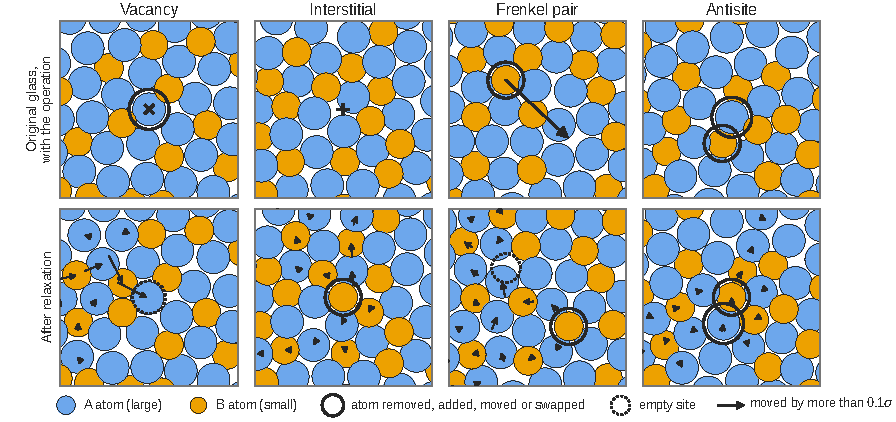
\includegraphics[width=0.64\linewidth]{figures/pd_fig1_defects.pdf}
\caption{The four point defects (the input of the finder). Top: the original glass and the operation ($\times$ removed, $+$ added, arrow: moved, two rings: species exchanged). Bottom: after relaxation; arrows show atoms moved by more than $0.1\sigma$. In the vacancy, neighbours have moved into the empty place.}
\label{fig:defects}
\end{figure}

We built the dataset ourselves~\citep{glassdefects2026} from the two-dimensional Kob--Andersen glass~\citep{kob1995,bruning2009}: 65\% large A and 35\% small B atoms with the pair potential
\begin{equation}
U=\sum_{i<j}\phi_{t_it_j}(r_{ij}),\qquad \phi_{ab}(r)=4\epsilon_{ab}\Big[\big(\tfrac{\sigma_{ab}}{r}\big)^{12}-\big(\tfrac{\sigma_{ab}}{r}\big)^{6}\Big],
\label{eq:potential}
\end{equation}
cut and shifted at $2.5\sigma_{ab}$, with $\epsilon_{AA}=1$, $\epsilon_{AB}=1.5$, $\epsilon_{BB}=0.5$, $\sigma_{AA}=1$, $\sigma_{AB}=0.8$, $\sigma_{BB}=0.88$. Here $r_{ij}$ is the distance between atoms $i$ and $j$ across the periodic box, $t_i\in\{A,B\}$ the species, and $\sigma=\sigma_{AA}$ the unit of length. With LAMMPS~\citep{thompson2022lammps} we melt $N=256$ atoms in a square periodic box of side $14.6\sigma$ at temperature $T=2$, cool at $10^{-2}$ per time unit to $T=0.01$ and minimise the energy. This gives 800 training, 100 validation and 100 test glasses. Each defect is made by one operation and the glass is relaxed again with the FIRE minimiser~\citep{bitzek2006fire} (Figure~\ref{fig:defects}): remove one atom (vacancy, 255 atoms); add a small B atom at the most open point within $2\sigma$ of a random position (interstitial, 257 atoms); move one atom to the most open point $1.2$--$3\sigma$ away (Frenkel pair); exchange an A atom and its nearest B atom (antisite). Each training glass gets 8 defects of each type (6,400 per type), each validation and test glass 2 (200 per type). A quarter of the Frenkel pairs undo themselves on relaxation (the moved atom pushes a same-species neighbour into the hole); we exclude them from the test, which leaves \pd{n-test} test defects.

\textbf{Physical checks of the data.} Every glass is relaxed until the largest force is below $10^{-8}$ (an energy minimum), with no two atoms closer than $0.56\sigma$. \pd{vacancy-open}\% of the vacancies stay more open than 95\% of the places in defect-free glass; in the rest, neighbours have moved in~\citep{bennett1979,delaye1993}. Frenkel pairs and antisites raise the energy in 91\% and 89\% of cases (medians $3.2\epsilon$ and $2.8\epsilon$). Assigning each atom to the nearest original site revealed the Frenkel pairs that had undone themselves (Section~\ref{sec:failures}).

\subsection{Problem definition}

A glass is $G=(X,t)$ with positions $X=(x_1,\dots,x_N)$, $x_i\in[0,L)^2$, and species $t$. The defected, relaxed glass is $\tilde G=(\tilde X,\tilde t)$ with $\tilde N$ atoms. Every atom has a \emph{role} $y_i\in\{0,\dots,4\}$: intact, next to an empty site, extra atom, displaced atom, wrong species, known from the operation. The \emph{finder} $f_\theta$ maps $\tilde G$ to role probabilities $P\in[0,1]^{\tilde N\times5}$. For a defect of type $k$ with role $c(k)$ it flags the atom $\hat\imath=\arg\max_i P_{i,c(k)}$. With $S$ the defect site(s) (both ends for a Frenkel pair or an antisite),
\begin{equation}
\text{found}=\mathbb 1\Big[\min_{s\in S}\lVert \tilde x_{\hat\imath}-s\rVert_L<1.5\sigma\Big],\qquad
\text{restored}=\mathbb 1\big[\operatorname{relax}(\operatorname{correct}_k(\tilde G,\hat\imath))\equiv G\big],
\label{eq:metrics}
\end{equation}
where $\lVert\cdot\rVert_L$ is the distance across the periodic box and $1.5\sigma$ covers the nearest neighbours (a random atom is that close only \pd{chance-min}--\pd{chance-max}\% of the time). $\operatorname{correct}_k$ adds an atom of the missing species at the most open point within $1.5\sigma$ of $\hat\imath$ (vacancy), removes $\hat\imath$ (interstitial), moves $\hat\imath$ to one of 8 nearby open points (Frenkel pair) or exchanges a neighbouring A--B pair (antisite); the type of defect is given. $\equiv$ means every original atom has an atom of its species within $0.05\sigma$, one to one.

\subsection{Model description}

\begin{figure}[t]
\centering
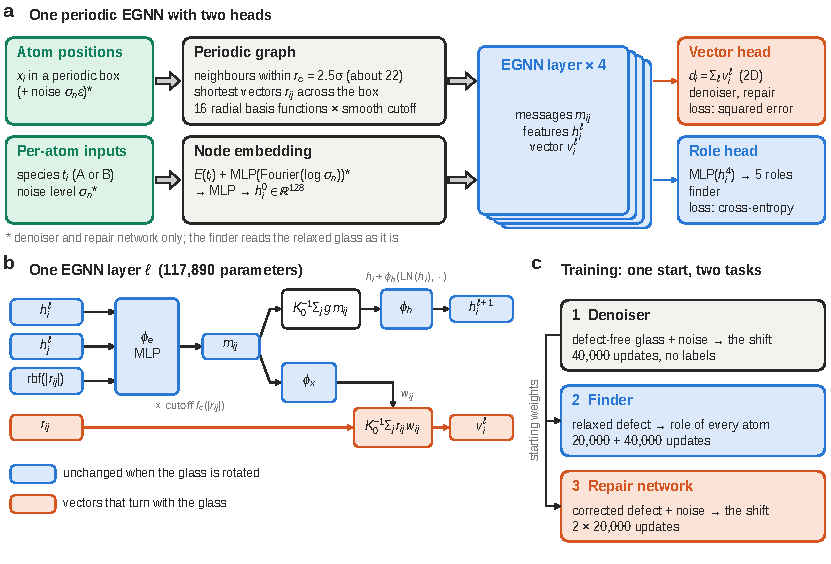
\includegraphics[width=0.84\linewidth]{figures/pd_fig4_network.pdf}
\caption{The model. (a)~One network: the positions define a periodic graph, the species (and, for the denoiser, the noise level) the starting features; four EGNN layers turn both into 128 features and a vector for every atom. The vector head gives the denoiser and the repair network, the role head the finder. (b)~One EGNN layer: blue quantities do not change when the glass is turned, orange ones turn with it. (c)~Training order: the denoiser first, without labels; its weights start the finder and the repair network.}
\label{fig:network}
\end{figure}

% Model description table of final_report.tex, laid out as Table 1 of Henderson et al.,
% Nucleic Acids Research 2019: model, hidden layers, parameters and hyper-parameters tried.
\begin{table}[t]
\centering
\caption{Deep learning models. The table shows the model architectures explored in this study, with the model name and hidden layers in columns 1 and 2. A repeated layer is written $N\times\{\text{layer}\}$, where $N$ is the number of repetitions; for example, $4\times\{\text{EGNN layer}\}$ means four EGNN layers in a row. Column 3 lists the parameters and hyper-parameters that were varied within each group, with the values tried in brackets; the value used for the final model is in bold. Fixed for all: 128 features, batches of 16 glasses, AdamW with learning rate $2\times10^{-4}$, gradient norm cut at 1, moving average of the weights 0.999. Output shapes and parameter counts are in Table~\ref{tab:shapes}.}
\label{tab:models}
\footnotesize\setlength{\tabcolsep}{4pt}
\begin{tabularx}{\linewidth}{@{}l>{\raggedright\arraybackslash}X>{\raggedright\arraybackslash}p{2.05in}@{}}
\toprule
Model & Hidden layers & Parameters/hyper-parameters \\
\midrule
4layerEGNN\_Denoiser & $1\times\{$embedding$\}$, $4\times\{$EGNN layer$\}$, vector head & Noise level $\sigma_n\sim\mathcal U(0.001,1)$; updates (40,000) \\
\addlinespace
4layerEGNN\_Finder & $1\times\{$embedding$\}$, $\mathbf{4}\times\{$EGNN layer$\}$, $1\times\{$Dense 128, Dense 5$\}$ & Starting weights (\textbf{denoiser}, random) \\
2layerEGNN\_Finder & $1\times\{$embedding$\}$, $2\times\{$EGNN layer$\}$, $1\times\{$Dense 128, Dense 5$\}$ & Class weights $w_c$ (\textbf{frequency}$^{\mathbf{-1/2}}$, none) \\
1layerEGNN\_Finder & $1\times\{$embedding$\}$, $1\times\{$EGNN layer$\}$, $1\times\{$Dense 128, Dense 5$\}$ & Frenkel pairs in training (\textbf{all}, real only) \\
 & & Updates (2,000, 20,000, \textbf{60,000}) \\
 & & Learning rate after 20,000 updates ($2\times10^{-4}$, $\mathbf{1\times10^{-4}}$) \\
 & & Calibration (none, \textbf{logit adjustment}); seeds (\textbf{0}, 1, 2) \\
\addlinespace
4layerTransformer\_Finder & $1\times\{$embedding$\}$, $4\times\{$attention with distance bias (8 heads), feed-forward$\}$, $1\times\{$Dense 128, Dense 5$\}$ & Starting weights (random); learning-rate warm-up (1,000 updates); updates (20,000); seeds (0, 1, 2) \\
5levelUNet\_Finder & $1\times\{$draw glass as picture$\}$, $5\times\{$Conv, Conv, pooling$\}$, $4\times\{$upsample, Conv, Conv$\}$, $1\times\{$Dense 64, Dense 5$\}$ & Starting weights (random); training augmentation (8 turns and mirrors, random shift); test-time average over 8; updates (20,000); seeds (0, 1, 2) \\
\addlinespace
4layerEGNN\_Repair & as 4layerEGNN\_Denoiser & Weight of displaced atoms (1, \textbf{11}); noise level ($\mathcal U(0.001,0.5)$, \textbf{log-uniform (0.001, 0.3)}); updates ($2\times20{,}000$) \\
\bottomrule
\end{tabularx}
\end{table}

% written by make_final_numbers.py
\begin{table}[t]
\centering
\caption{Output shape and number of parameters of every block, for one batch of 16 glasses of 256 atoms (shapes: glasses $\times$ atoms $\times$ features; for the CNN: glasses $\times$ channels $\times$ pixels $\times$ pixels). The neighbour graph holds up to 64 neighbours per atom (about 22 are within the cutoff). Measured on the trained networks.}
\label{tab:shapes}
\scriptsize\setlength{\tabcolsep}{4pt}
\begin{tabularx}{\linewidth}{@{}>{\raggedright\arraybackslash}Xlr@{}}
\toprule
Block & Output shape & Parameters \\
\midrule
\multicolumn{3}{@{}l}{\emph{EGNN finder} (the denoiser is the same with a noise-level input and the vector head)} \\
Input: positions, species & $16\times256\times2$, $16\times256$ & 0 \\
Neighbour graph and distance features (16 radial functions) & $16\times256\times64\times16$ & 0 \\
Input embedding (denoiser: with noise level) & $16\times256\times128$ & 34,304 (59,136) \\
$4\times$\{EGNN layer\}: features $h$, vector $v$ & $16\times256\times128$, $16\times256\times2$ & $4\times117,890$ \\
Role head \{Dense 128, Dense 5\} (denoiser: vector head, sum of $v$) & $16\times256\times5$ ($16\times256\times2$) & 17,157 (0) \\
\emph{Total} & & 523,021 (530,696) \\
\addlinespace
\multicolumn{3}{@{}l}{\emph{Transformer finder}} \\
Embedding: species, and neighbours of each species by distance & $16\times256\times128$ & 20,992 \\
Pair features from every distance (32 radial functions) & $16\times256\times256\times64$ & 6,272 \\
$4\times$\{attention with distance bias (8 heads), feed-forward 256\} & $16\times256\times128$ & $4\times133,000$ \\
Layer norm, role head \{Dense 128, Dense 5\} & $16\times256\times5$ & 17,413 \\
\emph{Total} & & 576,677 \\
\addlinespace
\multicolumn{3}{@{}l}{\emph{CNN finder} (U-Net)} \\
Glass drawn as a picture, one channel per species & $16\times2\times128\times128$ & 0 \\
Encoder: $5\times$\{Conv $3\times3$, Conv $3\times3$\}, average pooling between levels & $16\times\{16, 32, 48, 64, 96\}\times\{128, 64, 32, 16, 8\}^2$ & 255,264 \\
Decoder: $4\times$\{upsample, join skip, Conv $3\times3$, Conv $3\times3$\} & $16\times\{64, 48, 32, 16\}\times\{16, 32, 64, 128\}^2$ & 240,576 \\
Read at each atom, add species; role head \{Dense 64, Dense 5\} & $16\times256\times5$ & 2,469 \\
\emph{Total} & & 498,309 \\
\bottomrule
\end{tabularx}
\end{table}


All models are listed in Table~\ref{tab:models}; Table~\ref{tab:shapes} gives the output shape and parameters of every block, and Figure~\ref{fig:network} the structure. The main network is a periodic EGNN~\citep{satorras2021egnn}. Atoms closer than $r_c=2.5\sigma$ are linked; $r_{ij}$ is the shortest vector between them across the box, expanded in 16 Gaussian radial functions (rbf) with a smooth cutoff $f_c$. Starting from an embedding of the species, $h_i^0=\mathrm{MLP}(E(t_i))\in\mathbb R^{128}$ with $E$ a learned table (the denoiser adds 64 random Fourier features of $\log\sigma_n$), each of four layers computes
\begin{equation}
\begin{aligned}
m_{ij}&=\phi_e\big(h_i,h_j,\mathrm{rbf}(|r_{ij}|)\big)f_c(|r_{ij}|),\qquad
h_i\leftarrow h_i+\phi_h\Big(\mathrm{LN}(h_i),\tfrac{1}{K_0}\textstyle\sum_j g(m_{ij})m_{ij}\Big),\\
v_i^\ell&=\tfrac{1}{K_0}\textstyle\sum_j r_{ij}\,\phi_x(m_{ij})f_c(|r_{ij}|),
\end{aligned}
\label{eq:layer}
\end{equation}
with two-layer networks $\phi_e,\phi_h,\phi_x$ (SiLU), a sigmoid gate $g$, layer normalisation LN and $K_0=24$. The features $h_i$ depend only on distances and species, so the role probabilities do not change when the glass is shifted, turned or renumbered. The vector $d_i=\sum_\ell v_i^\ell$ turns with the glass and has the form of a force; it is the output of the denoiser. The finder's role head is $P_i=\operatorname{softmax}\big(W_2\,\mathrm{SiLU}(W_1h_i^4)\big)$ with $W_1\in\mathbb R^{128\times128}$, $W_2\in\mathbb R^{5\times128}$. Four layers reach $10\sigma$, more than half of the $14.6\sigma$ box.

\textbf{Transformer finder.} Each atom starts from its species and its surroundings, $h_i^0=E(t_i)+\mathrm{MLP}(\rho_i)$, where $\rho_i\in\mathbb R^{2\times16}$ counts the neighbours of each species within $2.5\sigma$ in 16 Gaussian distance bins. Every pair of atoms gets features $e_{ij}=\mathrm{MLP}(\mathrm{rbf}_{32}(|r_{ij}|))\in\mathbb R^{64}$ from its distance across the box. Each of four blocks computes, for 8 heads $k$ of 16 dimensions,
\begin{equation}
a^{k}_{ij}=\operatorname{softmax}_j\Big(\tfrac{1}{4}\,q_i^{k}\cdot \kappa_j^{k}+w_k^\top e_{ij}+c_k\Big),\quad
h_i\leftarrow h_i+W_o\big[\textstyle\sum_j a^k_{ij}u_j^k\big]_{k=1}^{8},\quad
h_i\leftarrow h_i+\mathrm{FFN}(\mathrm{LN}(h_i)),
\label{eq:attention}
\end{equation}
where the queries, keys and values $q,\kappa,u$ are linear maps of $\mathrm{LN}(h)$ and FFN has 256 hidden units. The distance term $w_k^\top e_{ij}+c_k$ lets each head learn to look near or far. Only distances enter, so shifts, turns and renumbering change nothing; memory grows with $N^2$ (Table~\ref{tab:shapes}).

\textbf{CNN finder.} The glass is drawn as a two-channel picture, $I_s(p)=\sum_{i:\,t_i=s}\exp\big(-\lVert p-x_i\rVert_L^2/2b^2\big)$ for species $s$, on a $128\times128$ grid of pixel centres $p$ ($0.11\sigma$ per pixel, $b=0.15\sigma$), so positions finer than a pixel still show. A U-Net~\citep{ronneberger2015unet} with five levels (16 to 96 channels; at each level two $3\times3$ convolutions with group normalisation and SiLU; $2\times2$ average pooling on the way down, upsampling and skip connections on the way up) returns 16 features per pixel. Convolutions pad circularly, so the picture wraps around like the box. The features at each atom are read by bilinear interpolation, joined to a species embedding and passed through a head $32\to64\to5$. Training applies one of the 8 quarter turns and mirror images of the square box and a random shift to each glass; testing averages the outputs over all 8.

\subsection{Losses and optimisation}

\textbf{Denoising (stage 1).} A defect-free glass $X_0$ is shifted by noise of size $\sigma_n\sim\mathcal U(0.001,1)$, $X=X_0+\sigma_n\varepsilon$ with $\varepsilon\sim\mathcal N(0,I)$, and the network predicts the shift:
\begin{equation}
\mathcal L_{\text{den}}(\theta)=\mathbb E_{X_0,\sigma_n,\varepsilon}\,\tfrac{1}{N}\textstyle\sum_i\big\lVert d_\theta(X,\sigma_n)_i-(x_i-x_{0,i})\big\rVert^2 .
\label{eq:den}
\end{equation}
Its minimiser is $d^*=-\sigma_n^2\nabla_X\log p_{\sigma_n}(X)$~\citep{vincent2011,efron2011}; in thermal equilibrium $\log p=-U/k_BT+\text{const}$, so $d^*$ points along the force $-\nabla U$. Our glasses are not in equilibrium, so we measured it: at $\sigma_n=0.05$ the learned correction and the true force agree with an average cosine of 0.81.

\textbf{Finding (stage 2).} The finder starts from the denoiser's weights and is trained with class-weighted cross-entropy over the atoms of a batch $B$:
\begin{equation}
\mathcal L_{\text{find}}(\theta)=-\frac{\sum_{i\in B} w_{y_i}\log P_\theta(y_i\mid\tilde G)_i}{\sum_{i\in B} w_{y_i}},\qquad w_c=(n_c/n_0)^{-1/2},
\label{eq:find}
\end{equation}
where $n_c$ is the number of training atoms with role $c$; this gives $w=(1, 9.2, 31.7, 31.8, 22.4)$, because over 98\% of the atoms are intact. The weights inflate the rare roles, so at test time we \emph{calibrate} by logit adjustment~\citep{menon2021}: $P_i=\operatorname{softmax}(z_i-\log w)$, with $z_i$ the network's outputs.

\textbf{Optimisation.} For every update with gradient $g=\nabla_\theta\mathcal L$, we cut the gradient norm, take an AdamW step~\citep{loshchilov2019adamw} and update a moving average of the weights:
\begin{equation}
g\leftarrow g\,\min\!\Big(1,\frac{c}{\lVert g\rVert_2}\Big),\quad
\theta\leftarrow\theta-\eta\,\frac{\hat m}{\sqrt{\hat v}+\epsilon},\quad
\bar\theta\leftarrow\beta\bar\theta+(1-\beta)\theta,
\label{eq:opt}
\end{equation}
with $c=1$; $\hat m,\hat v$ the bias-corrected running means of $g$ and $g^2$ ($\beta_1=0.9$, $\beta_2=0.999$, $\epsilon=10^{-8}$); weight decay 0; learning rate $\eta=2\times10^{-4}$ (finder: $10^{-4}$ for its last 40,000 updates; transformer: linear warm-up over 1,000 updates); $\beta=0.999$. All tests use $\bar\theta$.

\subsection{Training and evaluation procedure}
\label{sec:test}

\begin{enumerate}
\item \textbf{Batch sampling.} Each update draws one defect type with probability $1/4$ (a batch holds one type, since atom counts differ), then with probability 0.2 makes the batch defect-free (the originals, all intact), and draws 16 glasses of that type uniformly with replacement from the training split.
\item \textbf{Training.} Denoiser: 40,000 updates. Finder: 20,000 updates from the denoiser, then 40,000 at half the learning rate (0.2--0.3 s per update on one T4 GPU). We also trained two repair networks, 18 short finders (six settings $\times$ three seeds, 2,000 updates) and nine 20,000-update finders (three networks $\times$ three seeds), logging loss and gradient at every update.
\item \textbf{Validation.} Every 1,000 updates the moving-average model labels the first 200 validation defects of each type (uncalibrated); validation was used to choose settings and baseline rules, never test.
\item \textbf{Testing.} The final $\bar\theta$ flags one atom per test defect (calibrated). We report found and restored (Equation~\ref{eq:metrics}) per type. 95\% intervals come from 10,000 bootstrap resamples of the 100 test glasses. Methods are compared on the same defects with McNemar's exact test; for the twelve comparisons of each table (finder against three measures, four types) $p$ values are corrected with Holm's method~\citep{holm1979}.
\end{enumerate}

\section{Baselines and extensions}
\label{sec:baselines}

\textbf{Choice of baselines.} Each baseline flags one atom per defect and goes through the same correction and minimisation. \emph{Random atom} is the floor. \emph{Cell size} (Voronoi area, relative to the usual for the species) measures empty space~\citep{starr2002,laakkonen1988} without the potential. \emph{Unlike neighbours} (nearest neighbours of the other species) measures chemical order, which every defect disturbs in this mixture~\citep{kob1995}. \emph{Atom energy} (each atom's share of $U$) is the simplest measure that uses the potential, \emph{local pressure} the interstitial probe of~\citep{laakkonen1988}. The rule (largest, smallest or most unusual value) was chosen on validation glasses. \emph{True location given} is a reference for the repair. Deep learning baselines: the \emph{EGNN from random weights} isolates the effect of the denoising stage, and the \emph{transformer} and \emph{CNN} test whether a graph network is the right choice.

\begin{figure}[t]
\centering
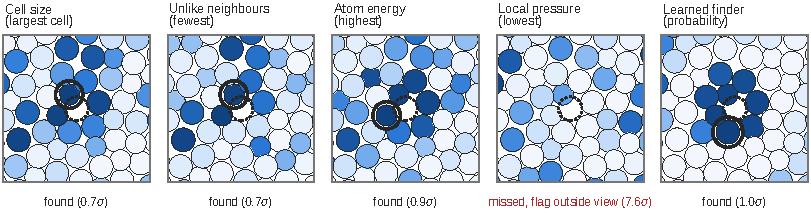
\includegraphics[width=\linewidth]{figures/fr_fig_baselines.pdf}
\caption{Original outputs of every method on the same test vacancy (dotted circle: where the atom was removed, not shown to the methods). Atoms are coloured by how suspicious each method finds them (rank within the glass, dark = most); the ringed atom is the one flagged. In this typical example three of the four measures also find the defect; local pressure flags an atom $7.6\sigma$ away.}
\label{fig:baselines}
\end{figure}

\textbf{Baseline output and reproduction.} Figure~\ref{fig:baselines} shows each baseline's output. The atom energy was computed by two separate programs, which agree on every defect; the per-atom pressures sum to the pressure of the box; the finder's evaluation gives the same rates on GPU and CPU; re-running a training with the same seed reproduces the weights exactly; and the denoiser reproduces the behaviour DM2 relies on, a correction along the true force (cosine 0.81).

\textbf{Extensions beyond DM2:} a role head, weighted loss and calibration make the denoiser a finder; the repair network removes a defect, not only noise; the benchmark compares measures and networks on exact labels.

\begin{figure}[tb]
\centering
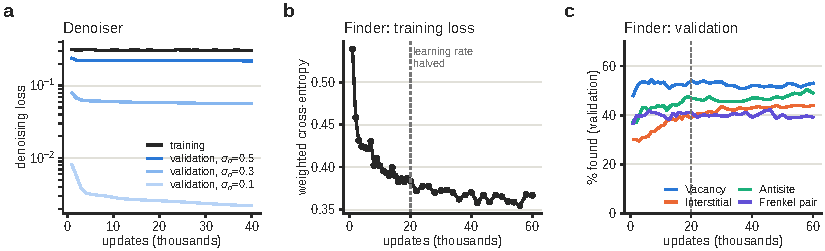
\includegraphics[width=\linewidth]{figures/fr_fig_training.pdf}
\caption{Training and validation. (a)~Denoiser: training loss (averaged over all noise levels, so it stays near the noise floor) and validation loss at three fixed noise levels. (b)~Finder: class-weighted training loss, mean over 1,000 updates. (c)~Finder: share of validation defects found (first 200 per type, uncalibrated, including the Frenkel pairs that undid themselves).}
\label{fig:training}
\end{figure}

\IfFileExists{fr_table_splits.tex}{% written by make_final_numbers.py
\begin{table}[t]
\centering
\caption{The finder of the main results on training, validation and test defects (real defects only). Loss: the class-weighted cross-entropy it was trained on, and the plain cross-entropy, per atom. Found (\%): calibrated, as everywhere in the results.}
\label{tab:splits}
\footnotesize\setlength{\tabcolsep}{4pt}
\begin{tabular}{@{}lrcccccccc@{}}
\toprule
 & & \multicolumn{2}{c}{Loss} & \multicolumn{5}{c}{Found (\%)} \\
\cmidrule(lr){3-4}\cmidrule(l){5-9}
Defects & $n$ & weighted & plain & Vacancy & Interst. & Antisite & Frenkel & All \\
\midrule
Training (200 per type) & 800 & 0.396 & 0.111 & 64.5 & 44 & 50.5 & 43 & 50.5 \\
Validation & 734 & 0.381 & 0.109 & 56.5 & 48.5 & 54.5 & 47.8 & 52.2 \\
Test & 750 & 0.371 & 0.109 & 69.5 & 50 & 49 & 45.3 & 54 \\
\bottomrule
\end{tabular}
\end{table}
}{}

\section{Results and analysis}
\label{sec:results}

\subsection{Training and validation}


The denoiser's validation loss keeps falling at small noise while its training loss is set by the noise itself (Figure~\ref{fig:training}a). The finder's training loss falls steeply over 10,000 updates; validation finding levels off after about 20,000 (Figure~\ref{fig:training}b,c); 40,000 more updates at half the learning rate raised the share of all test defects found from \pd{exp-20k}\% to \pd{exp-60k}\% (\pd{exp-p-length}). The finder does not overfit: it finds \pd{split-train-all}\% of training defects, \pd{split-val-all}\% of validation and \pd{split-test-all}\% of test defects, with similar losses (Table~\ref{tab:splits}).

\subsection{Finding and restoring on the test defects}

% written by make_final_numbers.py
\begin{table}[t]
\centering
\caption{Test results (\%). Found: the flagged atom lies within $1.5\sigma$ of the defect (for a Frenkel pair, of either end; the finder flags the displaced atom itself in \pd{frenkel-exact-finder}\%, the atom energy in \pd{frenkel-exact-energy}\%). Restored: the original glass is recovered after correcting the atoms at the flagged atom and minimising the energy. Brackets: 95\% intervals. Bold: the best method. Only the atom energy uses the potential to flag the atom; every repair ends with minimisation.}
\label{tab:found}\label{tab:restored}
\footnotesize\setlength{\tabcolsep}{3pt}
\begin{tabular}{@{}lcccccc@{}}
\toprule
Defect & $n$ & Learned finder & Cell size & Unlike neighb. & Atom energy & Reference \\
\midrule
\multicolumn{6}{@{}l}{\emph{Found}} & \emph{random atom} \\
Vacancy & 200 & \textbf{69.5} {\scriptsize[62, 76]} & 47.5 {\scriptsize[40, 55]} & 29 {\scriptsize[22, 36]} & 29.5 {\scriptsize[23, 36]} & 2.9 \\
Interstitial & 200 & \textbf{50} {\scriptsize[42, 57]} & 15 {\scriptsize[10, 20]} & 28 {\scriptsize[22, 34]} & 28 {\scriptsize[22, 34]} & 3 \\
Antisite & 200 & \textbf{49} {\scriptsize[42, 56]} & 16.5 {\scriptsize[12, 22]} & 31.5 {\scriptsize[25, 38]} & 29 {\scriptsize[23, 35]} & 4 \\
Frenkel pair & 150 & \textbf{45.3} {\scriptsize[38, 53]} & 26.7 {\scriptsize[20, 33]} & 27.3 {\scriptsize[21, 34]} & 32.7 {\scriptsize[25, 40]} & 5.4 \\
\addlinespace
\multicolumn{6}{@{}l}{\emph{Restored}} & \emph{true location given} \\
Vacancy &  & \textbf{53.5} {\scriptsize[46, 61]} & 40.5 {\scriptsize[34, 48]} & 22 {\scriptsize[16, 28]} & 26 {\scriptsize[20, 32]} & 67 {\scriptsize[60, 74]} \\
Interstitial &  & \textbf{38} {\scriptsize[31, 46]} & 8.5 {\scriptsize[4, 13]} & 21.5 {\scriptsize[16, 27]} & 21 {\scriptsize[16, 26]} & 80 {\scriptsize[74, 86]} \\
Antisite &  & \textbf{30} {\scriptsize[24, 36]} & 1.5 {\scriptsize[0, 4]} & 7.5 {\scriptsize[4, 11]} & 8 {\scriptsize[4, 12]} & 68.5 {\scriptsize[62, 74]} \\
Frenkel pair &  & \textbf{12.7} {\scriptsize[8, 18]} & 0 {\scriptsize[0, 2]} & 1.3 {\scriptsize[0, 3]} & 7.3 {\scriptsize[3, 11]} & 42 {\scriptsize[34, 50]} \\
\bottomrule
\end{tabular}
\end{table}



The finder finds more defects of every type than every classical measure (Table~\ref{tab:found}): \pd{lead-found-min}--\pd{lead-found-max} points more than the best measure for vacancies, interstitials and antisites ($\pd{p-worst-found}$ after Holm's correction), and \pd{found-finder-frenkel}\% against \pd{found-energy-frenkel}\% of Frenkel pairs ($p=\pd{p-found-energy-frenkel}$). Local pressure finds \pd{press-min}--\pd{press-max}\%, less than the atom energy and unlike neighbours for every type. Unlike neighbours find about as many as the atom energy, because an atom's energy follows its number of unlike neighbours (correlation $-0.90$ for A atoms): for finding, the potential adds little to a count. With the finder's flag, minimisation restores \pd{restored-finder-vacancy}\% of vacancies, \pd{restored-finder-interstitial}\% of interstitials and \pd{restored-finder-antisite}\% of antisites, more than every other route ($\pd{p-worst-restored}$; Table~\ref{tab:restored}). Given the true location it restores \pd{restored-ceiling-min}--\pd{restored-ceiling-max}\%: finding, not repair, limits the result. Can a network do the repair in place of the potential? A repair network trained to undo the defect (Table~\ref{tab:models}) moves the displaced atoms the right way: one step removes \pd{repair-removed-v2}\% of their error. But it adds nothing when minimisation follows, and on its own it breaks physical realism: after one step, \pd{repair-overlap-1}\% of the glasses (depending on the defect) have two atoms closer than ever occurs in the data, and after ten steps \pd{repair-overlap-10}\%. A network trained only on distances to a target does not know that atoms cannot overlap; the potential does.

\subsection{Design choices}

% written by make_report_numbers.py
\begin{table}[t]
\centering
\caption{Ablations of the finder: defects found (\%) on the real test defects after 2,000 updates, one setting changed per row. Every row is the mean of three training runs that differ only in the random seed; for all defects the spread between the three runs (standard deviation) follows the $\pm$. Size in millions of parameters. Difference: in all defects found, from the row it is compared with, run by run with the same seed; in brackets, in how many of the three runs the row was lower. The row compared with is the reference, or, for the two rows with fewer layers, the row with random starting weights and 4 layers.}
\label{tab:ablations}
\footnotesize\setlength{\tabcolsep}{3.2pt}
\begin{tabularx}{\linewidth}{@{}>{\raggedright\arraybackslash}Xcccccll@{}}
\toprule
Setting & Size & Vacancy & Interst. & Antisite & Frenkel & All & Difference \\
\midrule
Reference: starts from the denoiser, 4 layers, class weights & 0.52 & 63.0 & 30.7 & 41.7 & 38.7 & 43.8 $\pm$ 0.8 & -- \\
\addlinespace
Random starting weights & 0.52 & 14.3 & 26.8 & 24.2 & 22.2 & 21.9 $\pm$ 2.8 & $-$22.0 (3 of 3) \\
Random starting weights, 2 layers (reach $5\sigma$) & 0.29 & 13.8 & 26.5 & 20.8 & 21.3 & 20.6 $\pm$ 2.4 & $-$1.3 (3 of 3) \\
Random starting weights, 1 layer (reach $2.5\sigma$) & 0.17 & 12.3 & 21.8 & 14.2 & 13.8 & 15.6 $\pm$ 1.5 & $-$6.2 (3 of 3) \\
\addlinespace
No class weights & 0.52 & 63.2 & 31.0 & 39.5 & 35.1 & 42.7 $\pm$ 1.0 & $-$1.2 (3 of 3) \\
Trained without the Frenkel pairs that undid themselves & 0.52 & 64.7 & 30.8 & 40.2 & 38.0 & 43.8 $\pm$ 2.1 & 0.0 (2 of 3) \\
\bottomrule
\end{tabularx}
\end{table}

% written by make_report_numbers.py
\begin{table}[t]
\centering
\caption{Three kinds of network as finder: defects found (\%) on the real test defects. The first three rows were trained in exactly the same way, from random starting weights; each is the mean of three runs that differ in the random seed, with the spread between the runs after the $\pm$. The two rows below them are the EGNN that starts from the denoiser (one run each). Last row: the six transformer and CNN runs used together, by averaging their probabilities. Size in millions of parameters.}
\label{tab:finders}
\footnotesize\setlength{\tabcolsep}{3.2pt}
\begin{tabularx}{\linewidth}{@{}>{\raggedright\arraybackslash}Xlrccccccl@{}}
\toprule
Finder & Start & Updates & Runs & Size & Vacancy & Interst. & Antisite & Frenkel & All \\
\midrule
Transformer & random & 20,000 & 3 & 0.58 & 67.2 & 48.3 & 54.2 & 42.0 & 53.6 $\pm$ 0.3 \\
CNN & random & 20,000 & 3 & 0.50 & 69.7 & 51.2 & 52.8 & 38.4 & 54.0 $\pm$ 0.5 \\
\addlinespace
EGNN & random & 20,000 & 3 & 0.52 & 63.2 & 29.7 & 44.0 & 35.1 & 43.5 $\pm$ 0.5 \\
EGNN & denoiser & 20,000 & 1 & 0.52 & 67.0 & 47.5 & 46.5 & 36.7 & 50.3 \\
EGNN, main finder & denoiser & 60,000 & 1 & 0.52 & 69.5 & 50.0 & 49.0 & 45.3 & 54.0 \\
\addlinespace
Transformer + CNN, all six runs & random & 20,000 & 6 & -- & 70.0 & 49.5 & 56.0 & 41.3 & 55.1 \\
\bottomrule
\end{tabularx}
\end{table}


\begin{figure}[t]
\centering
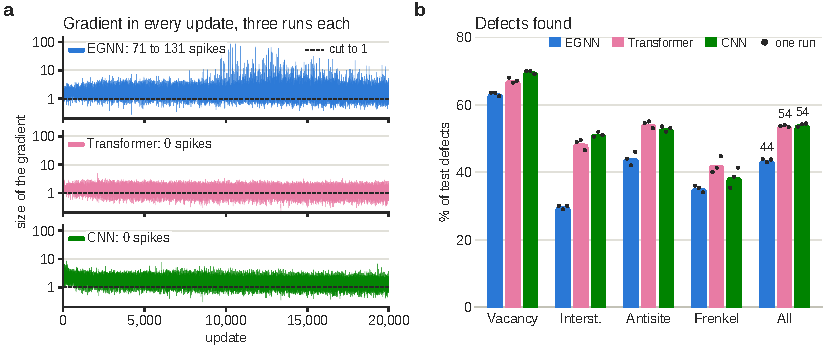
\includegraphics[width=0.86\linewidth]{figures/pd_fig5_finders.pdf}
\caption{Three kinds of network trained alike from random weights. (a)~Gradient norm at every update, before it is cut to 1 (dashed), three runs each; each step on the axis is a factor of ten. (b)~Test defects found: bars are means of three runs, dots single runs.}
\label{fig:finders}
\end{figure}

\textbf{Ablations} (Table~\ref{tab:ablations}, three seeds each, 2,000 updates). Starting from the denoiser doubles the defects found (\pd{abl-reference-all}\% against \pd{abl-scratch-all}\%, lower in all three seeds); after 20,000 updates the gap narrows (\pd{fin-pre-all}\% against \pd{fin-egnn-all}\%). One layer finds fewer than four (\pd{abl-layers1-all}\% against \pd{abl-scratch-all}\%). Removing the class weights or the Frenkel pairs that undid themselves changes little (a 2.6-point loss seen in one run was noise).

\textbf{Kind of network} (Table~\ref{tab:finders}, Figure~\ref{fig:finders}). Trained identically from random weights, the transformer finds \pd{fin-tr-all}\% and the CNN \pd{fin-cnn-all}\% of all test defects, the EGNN \pd{fin-egnn-all}\% (each ahead of the EGNN in every seed, \pd{fin-p-tr}); the gain is mostly in interstitials and antisites. Both match the main finder (\pd{fin-main-all}\%) with a third of its training and no denoising stage, and do not differ from each other (\pd{fin-p-tr-cnn}). \textbf{Stability:} the EGNN shows \pd{stab-egnn-gspikes} gradient spikes per 20,000-update run (gradient up to \pd{stab-egnn-largest}), the transformer and CNN none; with the cut at 1 no run failed, and three seeds of the same recipe find \pd{seed-ref-runs}\%.

\subsection{Failure modes}
\label{sec:failures}

\textbf{Frenkel pairs are poorly defined after relaxation.} Judged by which sites of the original glass are empty or doubly occupied, only \pd{fp-n-pair} of the 150 test Frenkel pairs are still Frenkel pairs; \pd{fp-n-anti} became antisite-like, \pd{fp-n-close} close pairs and \pd{fp-n-complex} complex. Of all 150, the finder flags the displaced atom itself in only \pd{frenkel-exact-finder}\% and restores \pd{restored-finder-frenkel}\%. \textbf{Some defects are hidden from every network:} \pd{fin-by-none}\% of the test defects are found by none of the three networks, and averaging all six transformer and CNN runs finds only \pd{fin-six-all}\%. \textbf{Small missing atoms defeat the classical measures:} the atom energy finds \pd{vacA-found-energy}\% of vacancies of A atoms but \pd{vacB-found-energy}\% of B atoms, while the finder finds both alike (\pd{vacA-found-finder}\% and \pd{vacB-found-finder}\%). \textbf{The finder says where, not whether:} on defect-free glasses its highest probability separates them from defected ones with an area under the ROC curve of only \pd{glass-auc}.

\subsection{What the finder has learned}

\begin{figure}[t]
\centering
\IfFileExists{figures/fr_fig_features.pdf}{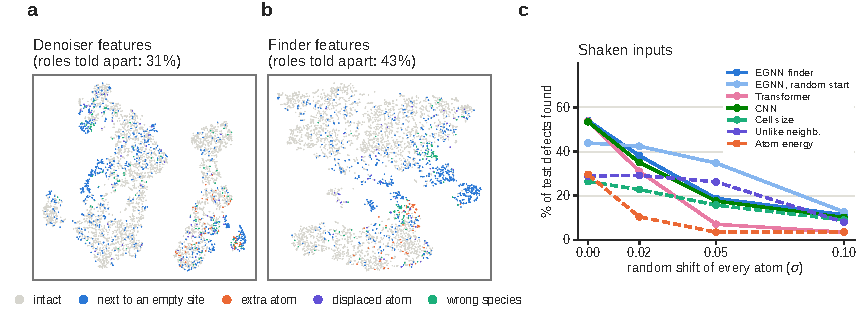
\includegraphics[width=\linewidth]{figures/fr_fig_features.pdf}}{\fbox{figure pending}}
\caption{(a,b)~The 128 features of \pd{feat-atoms} atoms of test glasses after the last layer (all atoms with a defect role and a sample of intact ones), embedded in two dimensions (t-SNE), coloured by true role: (a)~the denoiser, before any defect labels; (b)~the finder. The two large groups are the two species. In brackets: balanced accuracy of a 5-nearest-neighbour vote on the roles in the full 128 dimensions. (c)~Test defects found when every atom is shifted at random by a Gaussian of the given standard deviation.}
\label{fig:features}
\end{figure}

Figure~\ref{fig:features}a,b shows the atoms' learned features. In both maps the two large groups are the two species. In the denoiser's map, atoms of the defect roles are scattered among intact atoms. In the finder's map, part of the atoms next to an empty site form their own cluster and extra and wrong-species atoms gather together, but many defect atoms still sit among intact ones. A 5-nearest-neighbour vote on the 128 features tells the five roles apart with a balanced accuracy of \pd{knn-den}\% for the denoiser and \pd{knn-fin}\% for the finder (chance: 20\%): training on defects sharpens the features, but only partly.

\section{Discussion}
\label{sec:discussion}

\textbf{Significance.} A learned model reads relaxed point defects from the structure alone better than the four classical measures we tested, most of all where single-atom measures fail: small missing atoms, interstitials that have made room for themselves, and faults in chemical order. Noise-removal pre-training speeds up learning, but the kind of network matters more; all three networks miss the same third of the defects.

\textbf{Physical realism.} In both our studies a network that edits structure by itself breaks realism (Appendix~\ref{app:midterm}, Section~\ref{sec:results}); here every structure is an energy minimum, and the network only reads it.

\textbf{Sensitivity to input changes.} The EGNN and transformer give the same flagged atom when the glass is shifted, turned or renumbered (100\% of test glasses); the CNN changes its flag after a random shift in \pd{fin-cnn-noshift}\% of glasses, because a picture has pixels. Shaking every atom at random, as thermal vibration or measurement error would, hurts every method (Figure~\ref{fig:features}c). A shift of only $0.02\sigma$ lowers the finder from \pd{noise-fin-0}\% to \pd{noise-fin-20}\% (transformer and CNN alike) and the atom energy from \pd{noise-energy-0}\% to \pd{noise-energy-20}\%, because the energy rises steeply when two atoms come closer. The count of unlike neighbours does not change (\pd{noise-bonds-20}\%), nor much the EGNN trained from random weights (\pd{noise-scr-20}\%); at $0.1\sigma$ no method finds more than \pd{noise-max-last}\%. Trained only on perfectly relaxed glasses, the networks read fine detail of that structure, most of all the finder that starts from the denoiser.

\textbf{Risks and limitations.} (i) The defects are put in by hand; they are controlled test cases, not a picture of how faults arise in real glass, where atoms often move collectively~\citep{faupel2003}. (ii) The finder needs no potential once trained, but its training data come from one. (iii) One defect of known type per glass, in a two-dimensional model glass of 256 atoms at zero temperature; the interstitial is always a B atom. (iv) The main finder was trained once (the intervals cover the test sample only), and some development choices were made after earlier test results had been seen. (v) Slightly shaken atoms remove most of the networks' lead. Applied to real, noisy data, a finder could report confident but wrong defects.

\section{Future directions}

(1) Train on shaken inputs, so the finder stays robust when atoms vibrate. (2) Pre-train the transformer by noise removal and repair with all three finders. (3) Let the finder name the defect type and decide whether a glass has one, with labels from site occupancy. (4) Move to three-dimensional silica, where our model-free first stage shows finding to be the bottleneck again (76--96\% restored with the true location, 11--29\% found by coordination analysis).

\section{Conclusions}

With exact labels for the four standard point defects in a model glass, a denoising-pretrained graph network finds them from positions and species alone, \pd{lead-found-min}--\pd{lead-found-max} points better than the best classical measure (O1); correcting where it points and minimising restores up to \pd{restored-finder-vacancy}\% of the original glasses, with no learned repair network needed (O2). Training is stable with gradient clipping and repeatable to within a point; a transformer or CNN trained like the EGNN finds ten points more (O3). Finding remains the bottleneck for repair, and a random shift of $0.02\sigma$ already costs the main finder \pd{noise-drop-fin} points.

\section*{Contributions}
{\footnotesize\setlength{\tabcolsep}{4pt}
\begin{tabularx}{\linewidth}{@{}l>{\raggedright\arraybackslash}Xl@{}}
\toprule
Workstream & What it covers & Member \\
\midrule
Data and physics & glass generation, potential, relaxation, physical checks of the defects & Nicholaus Ladislaus \\
Defects and evaluation & defect operations, success tests, baselines, statistics & Stacy Cheruto \\
Models and training & denoiser, finder, repair network, transformer and CNN; training runs & Abubakar Chilala \\
Repair procedure & correction steps, choice of gap and pair, repair without a potential & Gentille Uwera \\
Baselines and writing & figures, reports & Michel Sangwa \\
Supervision & course teaching assistant; supervised the project & Boniface Godwin \\
\bottomrule
\end{tabularx}}

\paragraph{Acknowledgements.} We thank Prof.\ Ismaila Dabo (Materials Science and Engineering, Carnegie Mellon University) for the review that redirected this project.

\paragraph{Code and data.} {\raggedright Code, dataset, trained models and every number in this report: \repo{} (branch \path{dabo-point-defects}); the analyses specific to this report are in \path{scripts/pilots/final_report_analysis.py} and \path{results/final_report_20261117/}.\par}

\bibliographystyle{abbrvnat}
{\small\bibliography{refs}}

\appendix
\section{Response to the midterm review}
\label{app:midterm}

Table~\ref{tab:midterm} answers each point of the reviews of our midterm report. The numbers in rows 2--4 are from the midterm study (placing self-defined defects D1$-$, D1+ and D2 with a guided diffusion model), whose code and results are on the branch \path{main} of the repository; D2 is a small B atom with at least two B neighbours within $1.2\sigma$, D1+ an A atom with at least 8 neighbours.

\begin{table}[h]
\centering
\caption{The reviewers' points and how this report answers them. W$_1$: distance between the distribution of atom energies around the placed defects and around natural ones (natural floor 0.013).}
\label{tab:midterm}
\footnotesize\setlength{\tabcolsep}{4pt}
\begin{tabularx}{\linewidth}{@{}>{\raggedright\arraybackslash}p{1.45in}>{\raggedright\arraybackslash}X@{}}
\toprule
Point raised & What we did or found \\
\midrule
Writing too terse; more detail on the architecture & Every network is described layer by layer with its equations (Section~\ref{sec:method}, Equations~\ref{eq:layer}--\ref{eq:attention}); Table~\ref{tab:models} lists the layers and the hyper-parameters tried, Table~\ref{tab:shapes} the output shape and parameters of every block, Figure~\ref{fig:network} the structure. \\
\addlinespace
Trade-off between placement success and realism under stronger guidance & Measured: for D2, raising the guidance weight from 2 to 6 raised success after relaxation from 0.56 to 0.79, but W$_1$ grew from 0.056 to 0.089, as far from natural as hand insertion (0.087). Stronger guidance buys success with realism. \\
\addlinespace
Why D1+ defects remain difficult & Natural D1+ sites survive noise and relaxation in their own glass (99--100\%), but transplanted into another glass with their 47 nearest atoms they relax away in 97\% of cases. An over-coordinated atom is held in place by its host beyond $3.5\sigma$, so no method that edits a small region can place it. \\
\addlinespace
Strengthen physical validation before 3D silica & Midterm study: in 50-time-unit simulations at temperature 0.01, generated D2 defects kept their identity in 83\% of runs, hand-inserted ones in 94\% and natural ones in 100\% (at temperature 0.1: 73\%, 80\%, 88\%). This study: every structure is an energy minimum, each defect type is checked physically (Section~\ref{sec:method}), and the silica stage so far uses no learned model. \\
\addlinespace
Can the model reliably make a requested defect while keeping the material realistic and stable? & Not reliably (rows above). With Prof.\ Dabo's point that standard defects can be made without learning, we now make defects with physics and use learning to find them. A network that edits structure itself (the repair network) again breaks realism (Section~\ref{sec:results}). \\
\bottomrule
\end{tabularx}
\end{table}

\end{document}
